\documentclass[twoside]{article}
\usepackage{fullpage}
\usepackage[pdftex]{graphicx}
\usepackage{wrapfig}
\usepackage{amsmath}
\usepackage{hyperref}
\usepackage{sectsty}
%\sectionfont{\fontsize{13}{15}\selectfont}
\usepackage{fixltx2e}
\usepackage{fancyhdr}
\pagestyle{fancy}
\fancyhead{}
\fancyfoot{}
\renewcommand{\headrulewidth}{0pt}
\fancyfoot[R] {\thepage}
\newenvironment{code}{\fontfamily{lmtt}\selectfont}{}
\date{}


\begin{document}
\title{CSI 370 Computer Architecture Report\\ Data Structures with Advent of Code}
\author{Mason Lee \\
Champlain College\\
mason.lee@mymail.champlain.edu}
\maketitle

\begin{center}
    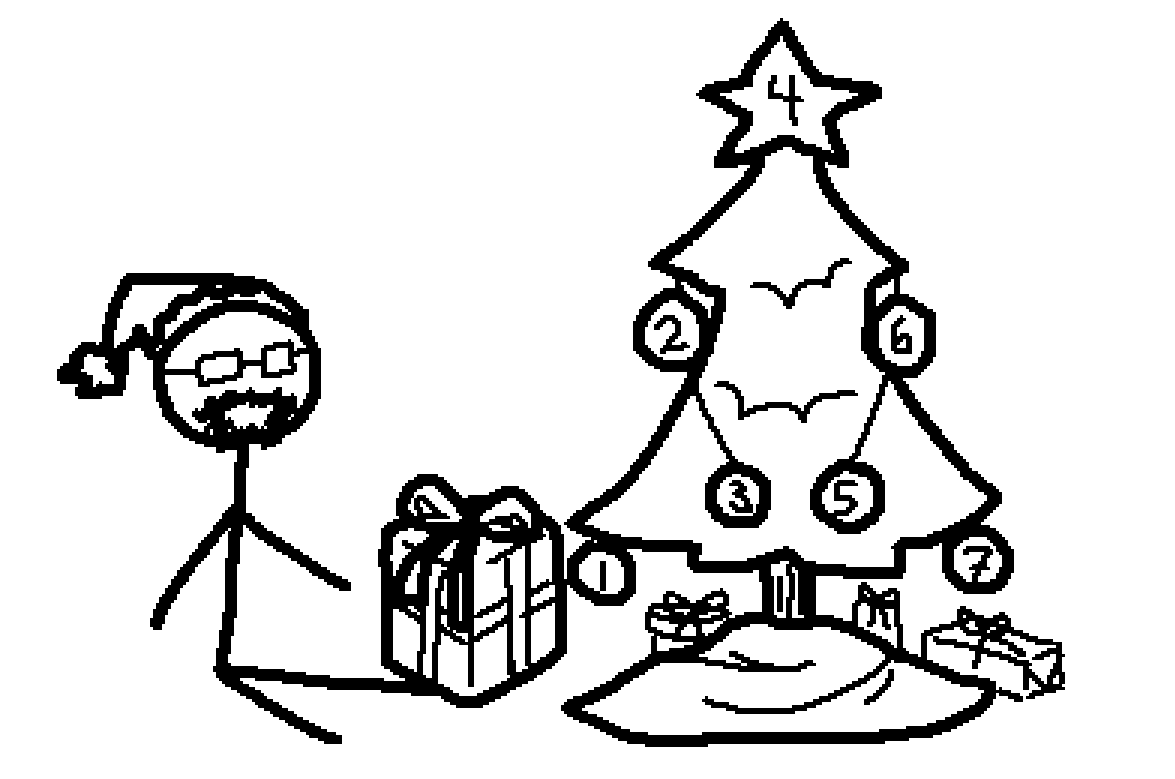
\includegraphics[width=.6\textwidth]{images/BrianHallChristmas.png}\\
\end{center}

\renewcommand{\labelitemi}{$\diamond$}
\noindent\textbf{\Large What?}\\
\noindent The project I chose to do is implementing data structures in Assembly. Specifically, I plan on implementing them in x64 masm. While this is an interesting project on its own, to give it a fun and unique spin, I use the data structures I implement to solve specific puzzles from Advent of Code. Advent of Code is an annual programming challenge event that takes place in December, containing a series of daily programming puzzles.  The difficulty of the problems varies from day to day, typically starting easier and getting progressively harder. One thing that many days have in common is that the “correct” solution may involve some sort of data structure. For instance, there may be a day when a good way to solve the puzzle is by using a stack, queue, or a tree of some sort. \\

\noindent For a better understanding of the puzzles I solved using the data structures I created, here are the two puzzles:
\begin{itemize}
    \item \href{https://adventofcode.com/2021/day/1}{2021 Day 1 Sonar Sweep}
    \item \href{https://adventofcode.com/2021/day/6}{2021 Day 6 Lanternfish}
\end{itemize}

\noindent The data structures I have implemented are:
\begin{itemize}
    \item Linked list
    \item Stacks
    \item Queues
\end{itemize}

\noindent \textbf{\Large Why?} \\
There are a couple of reasons I wanted to do this project specifically. First, I want to focus on a software-related project because I like the idea of working with software better than hardware. One of the things that draws me to computer science is the ability to create clean solutions to seemingly complex or tedious problems, which is frequently done using data structures. To have some sort of unique spin on the project of creating data structures, I wanted to apply it to something fun. Advent of Code is something that I do every year as a fun side project and I think it is a great way to practice coding skills as well as learn how to solve different types of problems. Another reason I started with the idea of data structures is that I wanted to learn how I can use dynamic memory allocation in low-level programming. \\

\noindent \textbf{\Large How?} \\
In this section I give a broad overview of some of the methods used to complete the project, however, a more in-depth explanation of the implementation of each data structure and puzzle will be in the “Implementation and Results” section. While I wanted to keep the project almost entirely in Assembly, I did use a little bit of C++ to help with certain tasks. The first thing that C++ was used for was the console output. Rather than relying on Assembly for string and integer output to the console the code often calls a C++ function. The second thing that C++ was used for is the file I/O required for handling Advent of Code input. For each Advent of Code puzzle, you get a huge text input that is specific to each user. To manage this, I keep the input in a text file and use C++ to get the data from the input file, which is then transferred over to the Assembly side where it can be loaded into different data structures. The bulk of this project is implementing data structures in Assembly using dynamic memory allocation. To accomplish this I use C’s malloc, and free functions to allocate different amounts of memory dynamically rather than keeping all data in variables. Malloc is a function that can dynamically allocate memory by passing in the number of bytes to allocate as a parameter, and free is a function that deallocates memory given a memory location. Member functions of data structures are also implemented in Assembly by passing the address of the head node in as the first parameter much like C++ does under the hood with the “this” keyword. \\

\noindent \textbf{\Large Challenges and Solutions} \\
Most of the challenges came from figuring out how to implement a data structure in Assembly. My original plan was to create a struct that acted as a single node. The struct would contain two quadwords, the first one to store the data at that node, and the second one to store the address of the next node. The plan was to use malloc to allocate memory, then create a new instance of a struct, and then move that struct into the newly allocated memory. While a version of this idea was used in the final implementation, it wasn’t the same. Because of the limitation of not being able to do 2 memory accesses in one command, it makes it difficult to create a struct and move it to a specific address. To mitigate this, I used what I know about structs to simulate a struct in memory. The way structs store their data is by allocating the total number of bytes stored in the struct, in this case with just two quadwords that’s 16 bytes for a single node. So I use the malloc function to allocate 16 bytes in memory and use the first 8 bytes to store the data of that node and the next 8 bytes to store the address of the next node, which by default is set to 0. For a visual representation of this, see Figure 1.
\begin{center}
    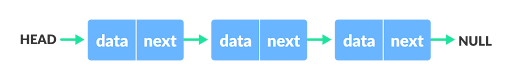
\includegraphics[width=.8\textwidth]{images/linkedList.png}\\
    Figure 1. Visual representation of a linked list
\end{center}

\noindent Another challenge that arose from using structs was trying to use a struct as a head node. This became an issue when trying to perform operations with the data structures, such as adding a new node or deleting the list using free. For instance, let’s say that we have a linked list with one element in it and the data that’s being stored in it is 0. Since there’s only one element in the list and the data is 0, that means that both the data and the next node would be set to 0. This is an issue because we have no way of distinguishing between a list that has no elements, and a list that has one element that is storing the value 0. To fix this, I made it so that the head node is only used for storing the address of the next node. This made it easier to be able to perform operations on a data structure without having to account for the first node being a struct that’s predefined in the data section.\\

\noindent Another issue that arose had to do with data types. Specifically, while I was solving day 6 part 2 there were some extraordinarily large numbers. When printed out using the C++ \_printInt function that I implemented this would cause the numbers to overflow and show up as seemingly random negative numbers. To fix this, I implemented a new function that did the same thing as \_printInt, except it takes in a long long int as the first parameter in order for the variable to be able to hold a big enough number. \\

\noindent \textbf{\Large Implementations and Results} \\\\
\noindent \textbf{\Large Data Structures} \\
\noindent The three data structures I implemented in this project were a linked list, a stack, and a queue. Because these three data structures have a lot in common I was able to take a lot of the functions I implemented for one and use it for the same functionality with a different data structure. For a recap of how each data structure was created from a macro stance refer back to the “Challenges and Solutions” section. In the following sections about data structures, I will talk about each of the “member” functions I implemented using Assembly.\\

\noindent \textbf{\Large Linked List} \\
\noindent Let’s start by briefly recapping how a linked list in this program is structured. Recall that a struct was used to define how a single node in the list is defined. Figure 2 shows the way the struct for a single linked list node was created. Remember that LLNode structs are not being stored at the memory locations, but instead, we allocate the amount of memory that would have been required for a struct to be stored at that location and then use pointer arithmetic to store the node’s data and the address of the next node in the corresponding addresses. \\
\begin{center}
    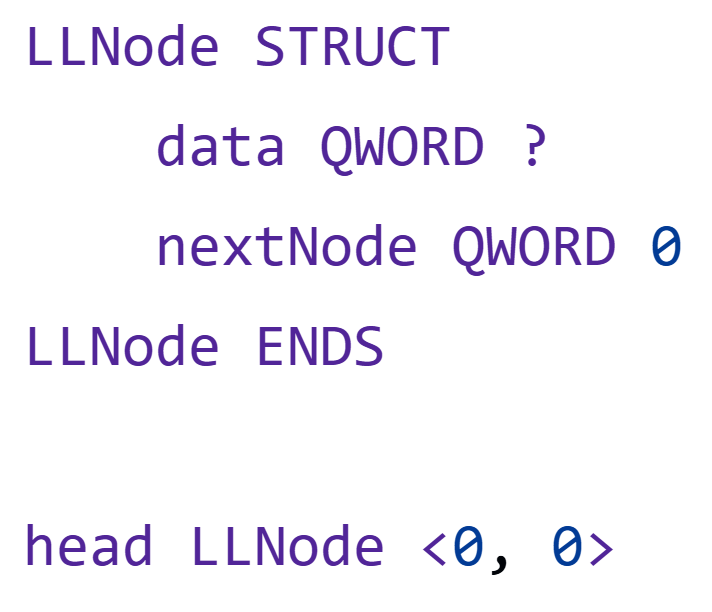
\includegraphics[width=.25\textwidth]{images/LLNodeStruct.png}\\
    Figure 2. Linked list node struct and head node declaration
\end{center}

\noindent \textbf{\large addNode} \\
\noindent The \_addNode function is potentially the most important function for this entire data structure. Without it, our linked list wouldn’t be able to hold any data! To accomplish this, the function takes in 2 parameters. The first parameter is passed in through rcx and is the memory address of the head node for our list. The second parameter is passed in through rdx and holds the value that will be added to the end of the linked list. For instance, if we wanted to add a new node to the end of the linked list and store the value 7 in it, we would load the address of the head node into rcx using lea, and we would move the value 7 into rdx, and then we would call \_addNode. Refer to Figure 3 for an example of how one would add a node to a linked list.
\begin{center}
    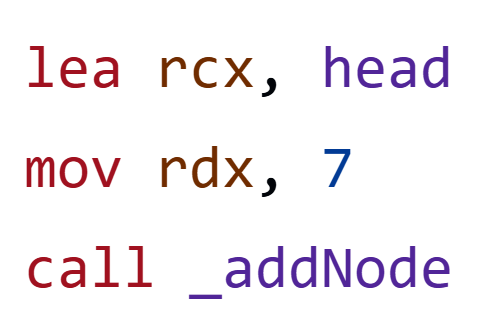
\includegraphics[width=.25\textwidth]{images/addNode.png}\\
    Figure 3. Adding a new node to a linked list
\end{center}

\noindent The way this code functions is very similar to how it would have been programmed in a high-level language. The first step in this function is to load the values stored in the head node into a new LLNode called currentNode. Throughout the function, currentNode is used to keep track of the node that we’re currently using. The next step is to continually move to the next node until the value of the next node is 0. To do this I use a series of jump statements essentially simulating a while loop. Once at the end of the list, we use malloc to allocate 16 bytes of memory and set the next node equal to the address that malloc returns. Then, we move to the next node which is the memory we just allocated, and we set the data at that node equal to the data that was passed into the function.
\begin{center}
    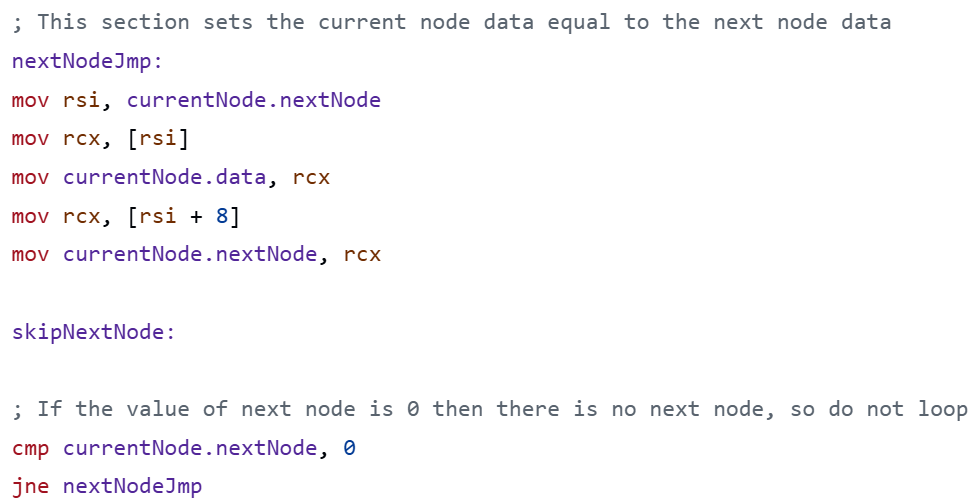
\includegraphics[width=.85\textwidth]{images/addNodeLoop.png}\\
    Figure 4. Looping through the linked list until nextNode equals 0
\end{center}

\noindent \textbf{\large printList} \\
\noindent The \_printList function is one that is shared across all three data structures and is mainly used for testing purposes. The way it works is very similar to the \_addNode function where it loops through each node in the linked list, however, instead of adding a node once it reaches the end of the list, at every node it will print out the data associated with that node using a C++ defined function called.
\begin{center}
    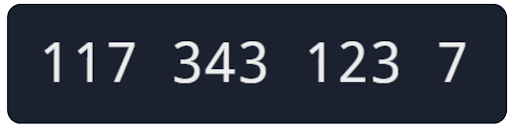
\includegraphics[width=.5\textwidth]{images/linkedListPrint.png}\\
    Figure 5. Example output of a linked list containing values 117, 343, 123, and 7
\end{center}

\noindent \textbf{\large getIndex \& setIndex} \\
\noindent The \_getIndex and \_setIndex functions work almost identically with the key difference being that \_getIndex returns the data stored at a certain value, and setIndex takes in a third parameter and sets the data at that index to the passed-in value. These functions use a loop to move forward a specified number of nodes rather than moving until the end. Once it reaches its desired node, in the case of \_getIndex, it will move the current data into the direct return register, rax, and return that value. In the case of \_setIndex, it changes the data that is stored at the specified index to the value that was passed into the r8 register. These functions are particularly useful when trying to edit any values in a linked list and are heavily relied on when solving Advent of Code 2021 day 6.\\

\noindent \textbf{\large deleteList} \\
\noindent Finally, the \_deleteList function is meant to be called at the end of every program to ensure that there are no memory leaks. This works similarly to the \_printList function except instead of printing the data stored at each index it will delete the previous node it visited. This means we have to keep track of the current node and the address of the previous node so we can call free on that address. Again, the importance of this function is not any sort of output or change being made to the list, it is cleaning up memory that we allocated using malloc to avoid any memory leaks in our program.\\\\


\noindent \textbf{\Large Stack} \\
\noindent The implementation of a stack in this project is similar to that of the implementation of a linked list. Some functions such as \_printList, \_addNode, and \_deleteList were able to be copied over exactly to the stack implementation with them being renamed to \_printStack, \_pushStack, and \_deleteStack. Recall that, stacks are first-in first-out data structures, meaning they have values pushed onto the end the same way that we added a new node to the end of our linked list, and they pop values off the top, meaning we remove the node at the end of the list. Another function that stacks typically have is a peek function which returns the data at the top of the stack.
\begin{center}
    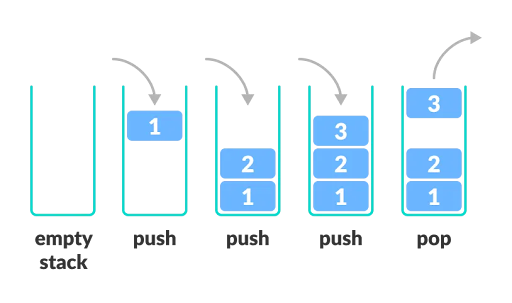
\includegraphics[width=.65\textwidth]{images/stackDiagram.png}\\
    Figure 6. Diagram of a stack
\end{center}

\noindent \textbf{\large popStack} \\
\noindent One of the unique functions of the stack for this project is the \_popStack function. This allows us to delete the last node that was pushed onto the stack and return the data that was stored in the last index. Once again, this acts very similarly to the linked list’s \_addNode function, except instead of adding a node to the stack at the end we set the second to last node’s nextNode to 0 and we call free on the address of the last node to effectively delete the node cleaning up our memory.
\begin{center}
    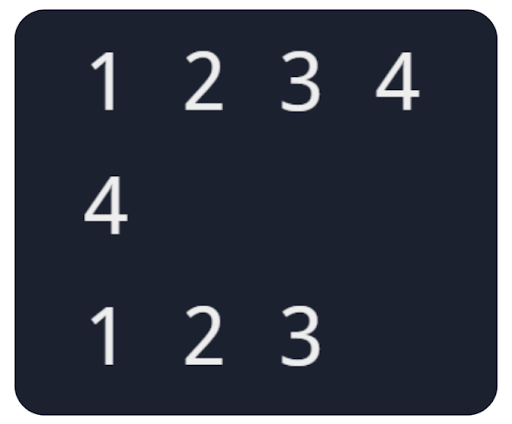
\includegraphics[width=.35\textwidth]{images/stackOutput.png}\\
    Figure 7. Stack being printed to console, followed by value popped off the stack, followed by the new stack
\end{center}

\noindent \textbf{\large peekStack} \\
\noindent The \_peekStack function is another that takes a lot of influence from the linked list’s \_addNode function, except at the end of the function it returns the data stored in the last node rather than adding a new node. Using the example in Figure 7, in the beginning, when calling \_peekStack on the original stack ([1, 2, 3, 4]) the peek function would return 4. After 4 had been popped off the stack if \_peekStack were called again it would return 3.\\\\


\noindent \textbf{\Large Queue} \\
\noindent A queue is a first-in first-out data structure meaning whatever the first node to be pushed onto the queue will be the next one to be popped off. In a traditional queue the functions to add and remove a node are called enqueue and dequeue, however in this program the functions are simply \_pushQueue and \_popQueue. Again, we were able to take some of the functions from previous data structures and implement them in the same way. These functions were the linked list’s \_addNode, \_printList, and \_deleteList functions which became \_pushQueue, \_printQueue, and \_deleteQueue respectively. Note that in Figure 8 nodes are added to the front of the queue at index 0. In my implementation, the nodes are all appended to the end of the queue, and when calling \_popQueue the node at index 0 is removed. This produces the same result, only backward, but is still a first-in-first-out data structure.
\begin{center}
    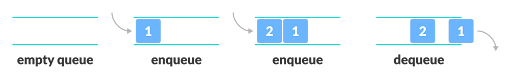
\includegraphics[width=.95\textwidth]{images/queueDiagram.png}\\
    Figure 8. Diagram of a queue
\end{center}

\noindent \textbf{\large popQueue} \\
\noindent The only unique function to a queue in this implementation is the \_popQueue function. To remove the first index we don’t have to do any traversal in the list. We simply replace the address at the “head node” with the second element of the queue, and call free on the address of the first element. After that, we return the data that was stored in the node that was just removed.
\begin{center}
    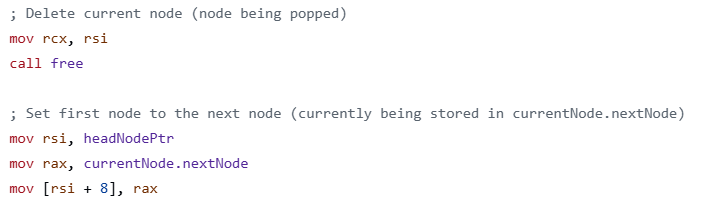
\includegraphics[width=.95\textwidth]{images/deleteNodeQueue.png}\\
    Figure 9. Code to delete the 0th node and replace the head node’s nextNode
\end{center}


\noindent \textbf{\Large Advent of Code Solutions} \\\\
\noindent \textbf{\large Day 1: Sonar Sweep} \\
\noindent The premise of the first day from 2021 is that you are in a submarine that performs a sonar sweep of the ocean floor. The sweep returns a report containing a list of integers each on a new line representing the ocean floor depth at different points. The goal is to figure out how quickly the depth increases, and to do that you have to count the number of times a depth measurement increases. See Figure 10 for a visualization of a test input being transformed into an answer.
\begin{center}
    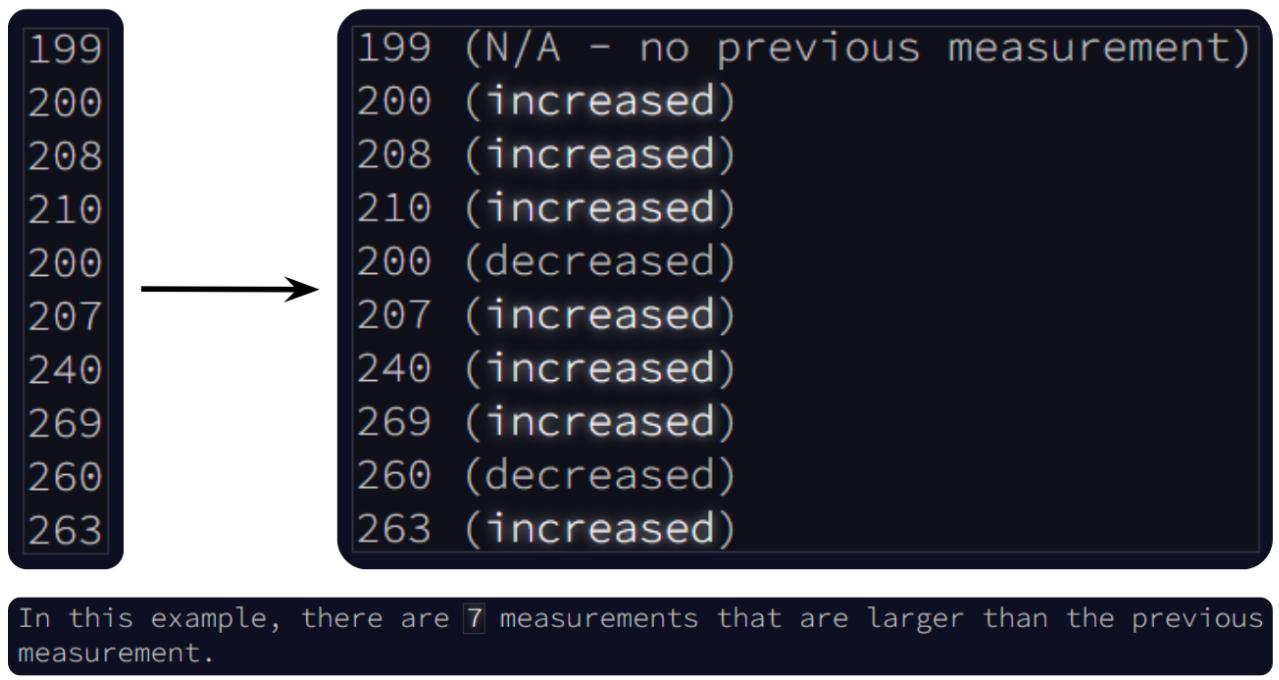
\includegraphics[width=.75\textwidth]{images/day01TestInput.png}\\
    Figure 10. Test input being transformed into an answer for part 1
\end{center}

\noindent In order to solve this problem we will be including the functions defined in LinkedList.asm and we will also be using a C++ function to get the data from SonarSweepDepths.txt (the puzzle input). The C++ function, \_getData, works as you would expect it to using regular C++ file I/O to go through the file by each new line, and it calls \_addNode to add a new node to our linked list of all of the recorded depths given to us by the puzzle input.
\begin{center}
    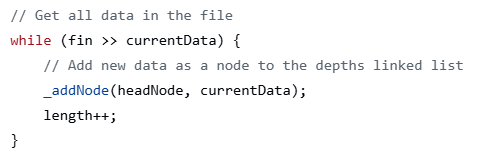
\includegraphics[width=.75\textwidth]{images/cppAddNodeLoop.png}\\
    Figure 11. C++ \_getData function adding new nodes to the linked list
\end{center}

\noindent Finally, to find the number of increases in the list, we loop through the linked list backward, and at each iteration, we check to see if the current node is greater than the data stored at the previous node. If it is then we do not increment the counter for the number of increases. Otherwise, we increment the counter for the number of increases. At the end, we print out our answer! The answer is shown in Figure 13.\\

\noindent \textbf{\large Part 2} \\
\noindent As mentioned before each puzzle has a part 2 that builds off the first part. Part 2 for this puzzle explains that considering every single measurement isn't as useful as you expected, so instead you decide to go with a sliding window approach, where you compare the sums of a three-measurement sliding window.
\begin{center}
    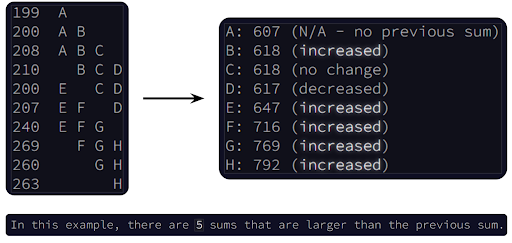
\includegraphics[width=.75\textwidth]{images/day01TestInputPart2.png}\\
    Figure 12.  Test input being transformed into an answer for part 2
\end{center}

\noindent The only real change from the part 1 solution to the part 2 solution is that in part 2 you’re comparing the number that is 3 indexes before the current index rather than the node behind the current node. This is because since two of the numbers are overlapping between windows, there’s no need to include them in a comparison.
\begin{center}
    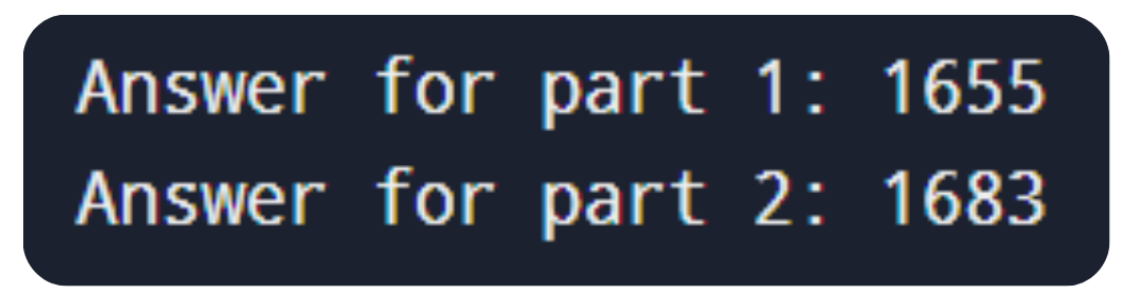
\includegraphics[width=.4\textwidth]{images/day01Output.png}\\
    Figure 13. Output for day 1 parts 1 and 2
\end{center}


\noindent \textbf{\large Day 6: Lanternfish} \\
\noindent Day 6 from 2021 has you model the exponential growth of a lanternfish population. The input is a list of integers separated by a comma. The integers represent an internal timer representing the number of days before the lanternfish reproduces. Once the timer goes below 0, their reproduction timer resets to 6 days and also creates a new lanternfish with an initial timer of 8 days. The question we’re asking is, how many lanternfish would there be after 80 days?
\begin{center}
    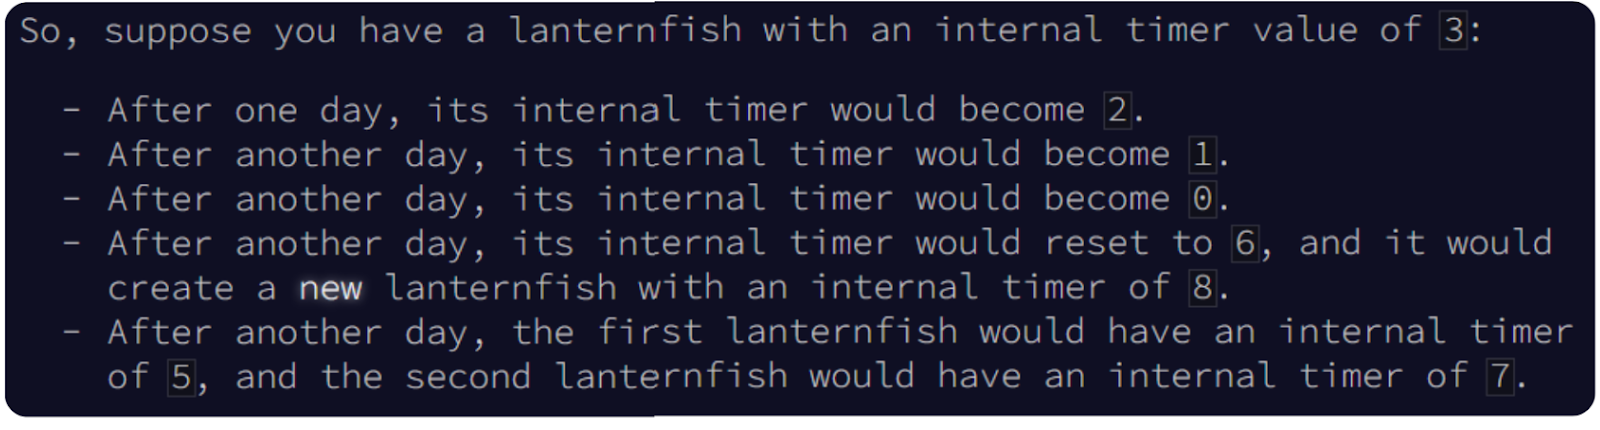
\includegraphics[width=.9\textwidth]{images/day06TestInput.png}\\
    Figure 14. Example for day 6
\end{center}

\noindent To solve this puzzle, we are going to use both a linked list and a queue. First, similarly to day 1, we use C++ file I/O to get all the initial fish timers into a linked list. From here, we load the number of fish with each timer into a queue. We then simulate a single day by popping a node from the queue, which represents the fish with 0 days left, adding the value that was just popped off to the number of fish with 6 days left to account for the internal timer of the fish resetting to six, and then pushing the value popped off back onto the queue to simulate creating the new fish. Let’s use an example, where there is a queue with the values [14, 22, 63, 34, 85, 6, 71, 28, 49]. The first index (14) represents the fish with 0 days left. That value is popped off the queue and appended to the end to represent the fish that were just created. The value is also added to the number of fish with 6 days left, which is currently 28 fish and turns into 42 fish. Our new fish queue is [22, 63, 34, 85, 6, 71, 42, 49, 14]. To get the total number of fish, we get the sum of the queue. For a visual representation of this, see Figure 15.
\begin{center}
    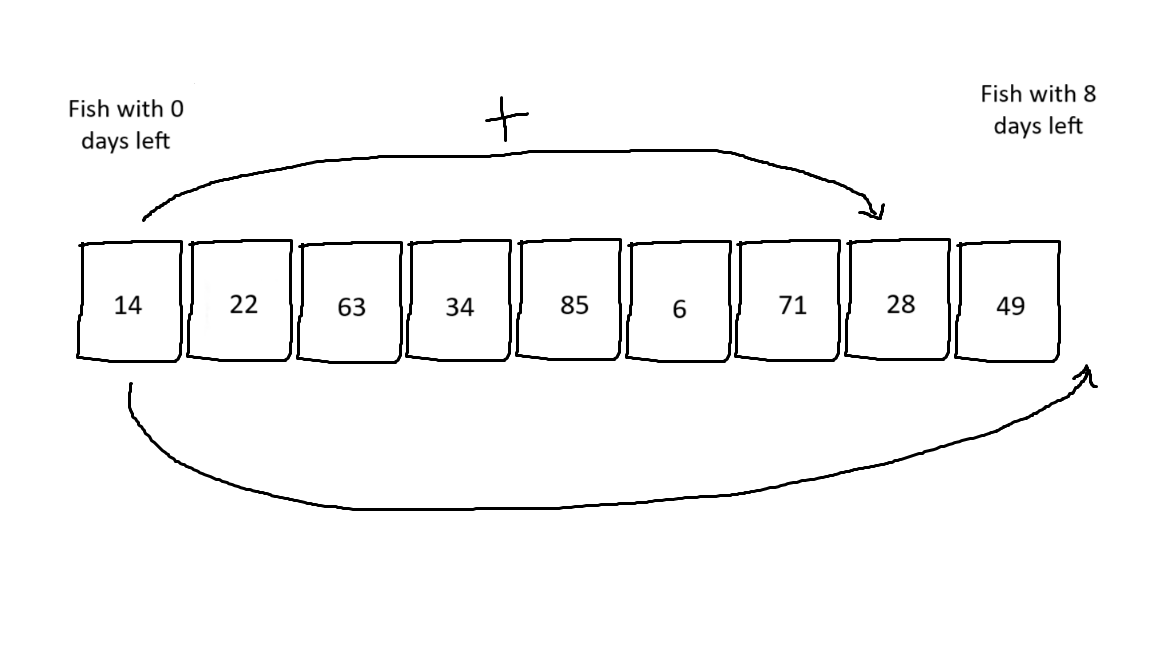
\includegraphics[width=.8\textwidth]{images/msPaintFishQueue.png}\\
    Figure 15. Simulating a single day using the fish queue
\end{center}

\noindent Coding this in assembly was made significantly easier with the use of the data structures that were implemented. Once we had the individual fish we were able to loop through each fish and add 1 to the correct index based on how many days that fish had left. I then made a function \_dayPass which updated the queue to reflect the changes made by a single day. I then used a loop to call this function 80 times to simulate the 80 days. After that, all that needed to be done was get the sum of the queue!\\

\noindent \textbf{\large Part 2} \\
\noindent Part 2 was very similar to part 1 with one minor difference. Instead of figuring out how many fish there are after 80 days, we are now looking for the number of fish after 256 days. Luckily, we already have a solution that is efficient enough for this not to matter. Given the results being way outside of the bounds of a 32-bit integer, I had to swap over to using long long ints instead as detailed in the Challenges and Solutions section. The only change that was made in part 2 was instead of calling \_dayPass 80 times, it was instead called 256 times.
\begin{center}
    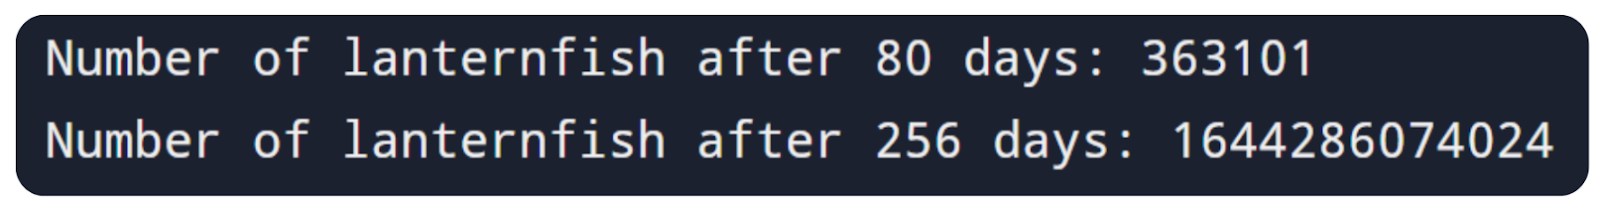
\includegraphics[width=.8\textwidth]{images/day06Output.png}\\
    Figure 16. Output for day 6 parts 1 and 2
\end{center}


\noindent \textbf{\Large Conclusion} \\
\noindent This project was originally supposed to contain one Advent of Code solution per data structure. In the end, I had the time to finish two puzzles from 2021. The first was Day 1 Sonar Sweep which used a linked list, and the second was Day 6 Lanternfish which used a queue to simulate an exponentially growing lanternfish population. While I wasn’t able to complete an Advent of Code puzzle that uses a stack due to time limitations I was still able to implement a stack and test it in Assembly. Overall, I’m happy with the contents of this project. Given more time I would love to create a tree in Assembly using some of the same methods.\\\\


\noindent \textbf{\Large Sources} \\
\begin{itemize}
    \item Hall, Brian R, and Kevin J Slonka. Assembly Programming and Computer Architecture for Software Engineers. Burlington Prospect Press, 2018.
    \item Fischer, Nicole. Brian Hall under the Binary Search Christmas Tree, 30 Nov. 2024.
    \item “Day 1 - Advent of Code 2021.” Adventofcode.com, \href{https://adventofcode.com/2021/day/1}{adventofcode.com/2021/day/1}
    \item “Day 6 - Advent of Code 2021.” Adventofcode.com, \href{https://adventofcode.com/2021/day/6}{adventofcode.com/2021/day/6}
    \item “Dynamic Memory Management - Cppreference.com.” Cppreference.com, 2022, \href{https://en.cppreference.com/w/c/memory}{en.cppreference.com/w/c/memory.} 
    \item Programiz. “LinkedList.” Www.programiz.com, \href{https://www.programiz.com/dsa/linked-list}{www.programiz.com/dsa/linked-list.}
    \item Programiz. “Stack.” Www.programiz.com, \href{https://www.programiz.com/dsa/stack}{www.programiz.com/dsa/stack.}
    \item “Queue Data Structure and Implementation in Java, Python and C/C++.” Www.programiz.com, \href{https://www.programiz.com/dsa/queue}{www.programiz.com/dsa/queue.} 
\end{itemize}

\end{document}